\documentclass[1p]{elsarticle_modified}
%\bibliographystyle{elsarticle-num}

%\usepackage[colorlinks]{hyperref}
%\usepackage{abbrmath_seonhwa} %\Abb, \Ascr, \Acal ,\Abf, \Afrak
\usepackage{amsfonts}
\usepackage{amssymb}
\usepackage{amsmath}
\usepackage{amsthm}
\usepackage{scalefnt}
\usepackage{amsbsy}
\usepackage{kotex}
\usepackage{caption}
\usepackage{subfig}
\usepackage{color}
\usepackage{graphicx}
\usepackage{xcolor} %% white, black, red, green, blue, cyan, magenta, yellow
\usepackage{float}
\usepackage{setspace}
\usepackage{hyperref}

\usepackage{tikz}
\usetikzlibrary{arrows}

\usepackage{multirow}
\usepackage{array} % fixed length table
\usepackage{hhline}

%%%%%%%%%%%%%%%%%%%%%
\makeatletter
\renewcommand*\env@matrix[1][\arraystretch]{%
	\edef\arraystretch{#1}%
	\hskip -\arraycolsep
	\let\@ifnextchar\new@ifnextchar
	\array{*\c@MaxMatrixCols c}}
\makeatother %https://tex.stackexchange.com/questions/14071/how-can-i-increase-the-line-spacing-in-a-matrix
%%%%%%%%%%%%%%%

\usepackage[normalem]{ulem}

\newcommand{\msout}[1]{\ifmmode\text{\sout{\ensuremath{#1}}}\else\sout{#1}\fi}
%SOURCE: \msout is \stkout macro in https://tex.stackexchange.com/questions/20609/strikeout-in-math-mode

\newcommand{\cancel}[1]{
	\ifmmode
	{\color{red}\msout{#1}}
	\else
	{\color{red}\sout{#1}}
	\fi
}

\newcommand{\add}[1]{
	{\color{blue}\uwave{#1}}
}

\newcommand{\replace}[2]{
	\ifmmode
	{\color{red}\msout{#1}}{\color{blue}\uwave{#2}}
	\else
	{\color{red}\sout{#1}}{\color{blue}\uwave{#2}}
	\fi
}

\newcommand{\Sol}{\mathcal{S}} %segment
\newcommand{\D}{D} %diagram
\newcommand{\A}{\mathcal{A}} %arc


%%%%%%%%%%%%%%%%%%%%%%%%%%%%%5 test

\def\sl{\operatorname{\textup{SL}}(2,\Cbb)}
\def\psl{\operatorname{\textup{PSL}}(2,\Cbb)}
\def\quan{\mkern 1mu \triangleright \mkern 1mu}

\theoremstyle{definition}
\newtheorem{thm}{Theorem}[section]
\newtheorem{prop}[thm]{Proposition}
\newtheorem{lem}[thm]{Lemma}
\newtheorem{ques}[thm]{Question}
\newtheorem{cor}[thm]{Corollary}
\newtheorem{defn}[thm]{Definition}
\newtheorem{exam}[thm]{Example}
\newtheorem{rmk}[thm]{Remark}
\newtheorem{alg}[thm]{Algorithm}

\newcommand{\I}{\sqrt{-1}}
\begin{document}

%\begin{frontmatter}
%
%\title{Boundary parabolic representations of knots up to 8 crossings}
%
%%% Group authors per affiliation:
%\author{Yunhi Cho} 
%\address{Department of Mathematics, University of Seoul, Seoul, Korea}
%\ead{yhcho@uos.ac.kr}
%
%
%\author{Seonhwa Kim} %\fnref{s_kim}}
%\address{Center for Geometry and Physics, Institute for Basic Science, Pohang, 37673, Korea}
%\ead{ryeona17@ibs.re.kr}
%
%\author{Hyuk Kim}
%\address{Department of Mathematical Sciences, Seoul National University, Seoul 08826, Korea}
%\ead{hyukkim@snu.ac.kr}
%
%\author{Seokbeom Yoon}
%\address{Department of Mathematical Sciences, Seoul National University, Seoul, 08826,  Korea}
%\ead{sbyoon15@snu.ac.kr}
%
%\begin{abstract}
%We find all boundary parabolic representation of knots up to 8 crossings.
%
%\end{abstract}
%\begin{keyword}
%    \MSC[2010] 57M25 
%\end{keyword}
%
%\end{frontmatter}

%\linenumbers
%\tableofcontents
%
\newcommand\colored[1]{\textcolor{white}{\rule[-0.35ex]{0.8em}{1.4ex}}\kern-0.8em\color{red} #1}%
%\newcommand\colored[1]{\textcolor{white}{ #1}\kern-2.17ex	\textcolor{white}{ #1}\kern-1.81ex	\textcolor{white}{ #1}\kern-2.15ex\color{red}#1	}

{\Large $\underline{12a_{0090}~(K12a_{0090})}$}

\setlength{\tabcolsep}{10pt}
\renewcommand{\arraystretch}{1.6}
\vspace{1cm}\begin{tabular}{m{100pt}>{\centering\arraybackslash}m{274pt}}
\multirow{5}{120pt}{
	\centering
	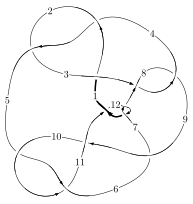
\includegraphics[width=112pt]{../../../GIT/diagram.site/Diagrams/png/891_12a_0090.png}\\
\ \ \ A knot diagram\footnotemark}&
\allowdisplaybreaks
\textbf{Linearized knot diagam} \\
\cline{2-2}
 &
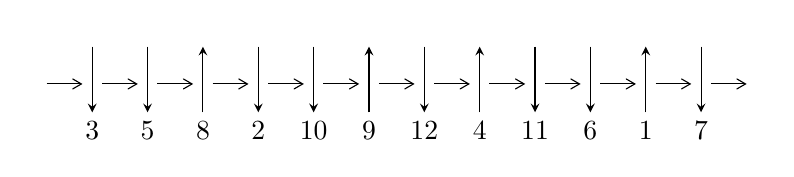
\begin{tikzpicture}[x=20pt, y=17pt]
	% nodes
	\node (C0) at (0, 0) {};
	\node (C1) at (1, 0) {};
	\node (C1U) at (1, +1) {};
	\node (C1D) at (1, -1) {3};

	\node (C2) at (2, 0) {};
	\node (C2U) at (2, +1) {};
	\node (C2D) at (2, -1) {5};

	\node (C3) at (3, 0) {};
	\node (C3U) at (3, +1) {};
	\node (C3D) at (3, -1) {8};

	\node (C4) at (4, 0) {};
	\node (C4U) at (4, +1) {};
	\node (C4D) at (4, -1) {2};

	\node (C5) at (5, 0) {};
	\node (C5U) at (5, +1) {};
	\node (C5D) at (5, -1) {10};

	\node (C6) at (6, 0) {};
	\node (C6U) at (6, +1) {};
	\node (C6D) at (6, -1) {9};

	\node (C7) at (7, 0) {};
	\node (C7U) at (7, +1) {};
	\node (C7D) at (7, -1) {12};

	\node (C8) at (8, 0) {};
	\node (C8U) at (8, +1) {};
	\node (C8D) at (8, -1) {4};

	\node (C9) at (9, 0) {};
	\node (C9U) at (9, +1) {};
	\node (C9D) at (9, -1) {11};

	\node (C10) at (10, 0) {};
	\node (C10U) at (10, +1) {};
	\node (C10D) at (10, -1) {6};

	\node (C11) at (11, 0) {};
	\node (C11U) at (11, +1) {};
	\node (C11D) at (11, -1) {1};

	\node (C12) at (12, 0) {};
	\node (C12U) at (12, +1) {};
	\node (C12D) at (12, -1) {7};
	\node (C13) at (13, 0) {};

	% arrows
	\draw[->,>={angle 60}]
	(C0) edge (C1) (C1) edge (C2) (C2) edge (C3) (C3) edge (C4) (C4) edge (C5) (C5) edge (C6) (C6) edge (C7) (C7) edge (C8) (C8) edge (C9) (C9) edge (C10) (C10) edge (C11) (C11) edge (C12) (C12) edge (C13) ;	\draw[->,>=stealth]
	(C1U) edge (C1D) (C2U) edge (C2D) (C3D) edge (C3U) (C4U) edge (C4D) (C5U) edge (C5D) (C6D) edge (C6U) (C7U) edge (C7D) (C8D) edge (C8U) (C9U) edge (C9D) (C10U) edge (C10D) (C11D) edge (C11U) (C12U) edge (C12D) ;
	\end{tikzpicture} \\
\hhline{~~} \\& 
\textbf{Solving Sequence} \\ \cline{2-2} 
 &
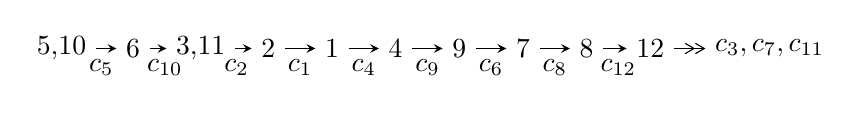
\begin{tikzpicture}[x=23pt, y=7pt]
	% node
	\node (A0) at (-1/8, 0) {5,10};
	\node (A1) at (1, 0) {6};
	\node (A2) at (33/16, 0) {3,11};
	\node (A3) at (25/8, 0) {2};
	\node (A4) at (33/8, 0) {1};
	\node (A5) at (41/8, 0) {4};
	\node (A6) at (49/8, 0) {9};
	\node (A7) at (57/8, 0) {7};
	\node (A8) at (65/8, 0) {8};
	\node (A9) at (73/8, 0) {12};
	\node (C1) at (1/2, -1) {$c_{5}$};
	\node (C2) at (3/2, -1) {$c_{10}$};
	\node (C3) at (21/8, -1) {$c_{2}$};
	\node (C4) at (29/8, -1) {$c_{1}$};
	\node (C5) at (37/8, -1) {$c_{4}$};
	\node (C6) at (45/8, -1) {$c_{9}$};
	\node (C7) at (53/8, -1) {$c_{6}$};
	\node (C8) at (61/8, -1) {$c_{8}$};
	\node (C9) at (69/8, -1) {$c_{12}$};
	\node (A10) at (11, 0) {$c_{3},c_{7},c_{11}$};

	% edge
	\draw[->,>=stealth]	
	(A0) edge (A1) (A1) edge (A2) (A2) edge (A3) (A3) edge (A4) (A4) edge (A5) (A5) edge (A6) (A6) edge (A7) (A7) edge (A8) (A8) edge (A9) ;
	\draw[->>,>={angle 60}]	
	(A9) edge (A10);
\end{tikzpicture} \\ 

\end{tabular} \\

\footnotetext{
The image of knot diagram is generated by the software ``\textbf{Draw programme}" developed by Andrew Bartholomew(\url{http://www.layer8.co.uk/maths/draw/index.htm\#Running-draw}), where we modified some parts for our purpose(\url{https://github.com/CATsTAILs/LinksPainter}).
}\phantom \\ \newline 
\centering \textbf{Ideals for irreducible components\footnotemark of $X_{\text{par}}$} 
 
\begin{align*}
I^u_{1}&=\langle 
-1.89807\times10^{152} u^{131}-2.61475\times10^{152} u^{130}+\cdots+9.05319\times10^{152} b+3.52721\times10^{153},\\
\phantom{I^u_{1}}&\phantom{= \langle  }6.80701\times10^{152} u^{131}+3.00477\times10^{153} u^{130}+\cdots+1.53904\times10^{154} a-7.27540\times10^{154},\\
\phantom{I^u_{1}}&\phantom{= \langle  }u^{132}+2 u^{131}+\cdots-19 u-17\rangle \\
I^u_{2}&=\langle 
b+1,\;2 u^8+u^7-5 u^6-3 u^5+4 u^4+3 u^3+2 u^2+a-2,\;u^9+u^8-2 u^7-3 u^6+u^5+3 u^4+2 u^3- u-1\rangle \\
I^u_{3}&=\langle 
6 u^3 a^2-2 a^2 u^2-2 u^3 a-3 a^2 u-11 u^2 a+9 u^3+2 a^2-4 a u+13 u^2+23 b+26 a-19 u-4,\\
\phantom{I^u_{3}}&\phantom{= \langle  }a^2 u^2-5 u^3 a+a^3-3 a^2 u-2 u^3-2 a^2+a u- u^2+a+2 u,\;u^4- u^2+1\rangle \\
\\
\end{align*}
\raggedright * 3 irreducible components of $\dim_{\mathbb{C}}=0$, with total 153 representations.\\
\footnotetext{All coefficients of polynomials are rational numbers. But the coefficients are sometimes approximated in decimal forms when there is not enough margin.}
\newpage
\renewcommand{\arraystretch}{1}
\centering \section*{I. $I^u_{1}= \langle -1.90\times10^{152} u^{131}-2.61\times10^{152} u^{130}+\cdots+9.05\times10^{152} b+3.53\times10^{153},\;6.81\times10^{152} u^{131}+3.00\times10^{153} u^{130}+\cdots+1.54\times10^{154} a-7.28\times10^{154},\;u^{132}+2 u^{131}+\cdots-19 u-17 \rangle$}
\flushleft \textbf{(i) Arc colorings}\\
\begin{tabular}{m{7pt} m{180pt} m{7pt} m{180pt} }
\flushright $a_{5}=$&$\begin{pmatrix}1\\0\end{pmatrix}$ \\
\flushright $a_{10}=$&$\begin{pmatrix}0\\u\end{pmatrix}$ \\
\flushright $a_{6}=$&$\begin{pmatrix}1\\u^2\end{pmatrix}$ \\
\flushright $a_{3}=$&$\begin{pmatrix}-0.0442288 u^{131}-0.195236 u^{130}+\cdots-4.35303 u+4.72722\\0.209657 u^{131}+0.288821 u^{130}+\cdots-0.869729 u-3.89610\end{pmatrix}$ \\
\flushright $a_{11}=$&$\begin{pmatrix}- u\\- u^3+u\end{pmatrix}$ \\
\flushright $a_{2}=$&$\begin{pmatrix}0.165429 u^{131}+0.0935846 u^{130}+\cdots-5.22276 u+0.831125\\0.209657 u^{131}+0.288821 u^{130}+\cdots-0.869729 u-3.89610\end{pmatrix}$ \\
\flushright $a_{1}=$&$\begin{pmatrix}-0.0596357 u^{131}-0.160770 u^{130}+\cdots+2.00581 u+2.68170\\0.0372237 u^{131}+0.0353922 u^{130}+\cdots-2.49460 u-2.42937\end{pmatrix}$ \\
\flushright $a_{4}=$&$\begin{pmatrix}-0.0650310 u^{131}-0.298884 u^{130}+\cdots-6.45305 u-3.27408\\-0.238080 u^{131}-0.407791 u^{130}+\cdots-3.33764 u+0.873239\end{pmatrix}$ \\
\flushright $a_{9}=$&$\begin{pmatrix}u^3\\u^5- u^3+u\end{pmatrix}$ \\
\flushright $a_{7}=$&$\begin{pmatrix}u^6- u^4+1\\u^8-2 u^6+2 u^4\end{pmatrix}$ \\
\flushright $a_{8}=$&$\begin{pmatrix}0.245372 u^{131}+0.352709 u^{130}+\cdots-0.795055 u-1.32177\\-0.0921465 u^{131}-0.0203027 u^{130}+\cdots+1.54595 u-1.62641\end{pmatrix}$ \\
\flushright $a_{12}=$&$\begin{pmatrix}-0.169720 u^{131}-0.238241 u^{130}+\cdots+2.75421 u+4.82837\\0.0461740 u^{131}+0.0537793 u^{130}+\cdots-1.73822 u-2.20458\end{pmatrix}$\\&\end{tabular}
\flushleft \textbf{(ii) Obstruction class $= -1$}\\~\\
\flushleft \textbf{(iii) Cusp Shapes $= 0.807591 u^{131}+1.32474 u^{130}+\cdots+3.73363 u-7.57808$}\\~\\
\newpage\renewcommand{\arraystretch}{1}
\flushleft \textbf{(iv) u-Polynomials at the component}\newline \\
\begin{tabular}{m{50pt}|m{274pt}}
Crossings & \hspace{64pt}u-Polynomials at each crossing \\
\hline $$\begin{aligned}c_{1}\end{aligned}$$&$\begin{aligned}
&u^{132}+62 u^{131}+\cdots+657 u+1
\end{aligned}$\\
\hline $$\begin{aligned}c_{2},c_{4}\end{aligned}$$&$\begin{aligned}
&u^{132}-14 u^{131}+\cdots+57 u-1
\end{aligned}$\\
\hline $$\begin{aligned}c_{3},c_{8}\end{aligned}$$&$\begin{aligned}
&u^{132}+u^{131}+\cdots-1024 u+512
\end{aligned}$\\
\hline $$\begin{aligned}c_{5},c_{10}\end{aligned}$$&$\begin{aligned}
&u^{132}+2 u^{131}+\cdots-19 u-17
\end{aligned}$\\
\hline $$\begin{aligned}c_{6}\end{aligned}$$&$\begin{aligned}
&u^{132}+6 u^{131}+\cdots-19963915 u-1325201
\end{aligned}$\\
\hline $$\begin{aligned}c_{7},c_{12}\end{aligned}$$&$\begin{aligned}
&u^{132}+2 u^{131}+\cdots-273 u-49
\end{aligned}$\\
\hline $$\begin{aligned}c_{9}\end{aligned}$$&$\begin{aligned}
&u^{132}+64 u^{131}+\cdots+2163 u+289
\end{aligned}$\\
\hline $$\begin{aligned}c_{11}\end{aligned}$$&$\begin{aligned}
&u^{132}-66 u^{131}+\cdots+6125 u+2401
\end{aligned}$\\
\hline
\end{tabular}\\~\\
\newpage\renewcommand{\arraystretch}{1}
\flushleft \textbf{(v) Riley Polynomials at the component}\newline \\
\begin{tabular}{m{50pt}|m{274pt}}
Crossings & \hspace{64pt}Riley Polynomials at each crossing \\
\hline $$\begin{aligned}c_{1}\end{aligned}$$&$\begin{aligned}
&y^{132}+30 y^{131}+\cdots+816247 y+1
\end{aligned}$\\
\hline $$\begin{aligned}c_{2},c_{4}\end{aligned}$$&$\begin{aligned}
&y^{132}-62 y^{131}+\cdots-657 y+1
\end{aligned}$\\
\hline $$\begin{aligned}c_{3},c_{8}\end{aligned}$$&$\begin{aligned}
&y^{132}-69 y^{131}+\cdots-21233664 y+262144
\end{aligned}$\\
\hline $$\begin{aligned}c_{5},c_{10}\end{aligned}$$&$\begin{aligned}
&y^{132}-64 y^{131}+\cdots-2163 y+289
\end{aligned}$\\
\hline $$\begin{aligned}c_{6}\end{aligned}$$&$\begin{aligned}
&y^{132}+32 y^{131}+\cdots-307315706207635 y+1756157690401
\end{aligned}$\\
\hline $$\begin{aligned}c_{7},c_{12}\end{aligned}$$&$\begin{aligned}
&y^{132}+66 y^{131}+\cdots-6125 y+2401
\end{aligned}$\\
\hline $$\begin{aligned}c_{9}\end{aligned}$$&$\begin{aligned}
&y^{132}+16 y^{131}+\cdots-345303 y+83521
\end{aligned}$\\
\hline $$\begin{aligned}c_{11}\end{aligned}$$&$\begin{aligned}
&y^{132}+14 y^{131}+\cdots-531353305 y+5764801
\end{aligned}$\\
\hline
\end{tabular}\\~\\
\newpage\flushleft \textbf{(vi) Complex Volumes and Cusp Shapes}
$$\begin{array}{c|c|c}  
\text{Solutions to }I^u_{1}& \I (\text{vol} + \sqrt{-1}CS) & \text{Cusp shape}\\
 \hline 
\begin{aligned}
u &= \phantom{-}0.938713 + 0.353789 I \\
a &= -0.912868 + 0.245129 I \\
b &= \phantom{-}0.852741 - 0.845895 I\end{aligned}
 & \phantom{-}3.55706 + 1.60482 I & \phantom{-0.000000 } 0 \\ \hline\begin{aligned}
u &= \phantom{-}0.938713 - 0.353789 I \\
a &= -0.912868 - 0.245129 I \\
b &= \phantom{-}0.852741 + 0.845895 I\end{aligned}
 & \phantom{-}3.55706 - 1.60482 I & \phantom{-0.000000 } 0 \\ \hline\begin{aligned}
u &= \phantom{-}0.996053 + 0.218414 I \\
a &= \phantom{-}0.806619 + 0.651472 I \\
b &= \phantom{-}0.655788 + 0.568246 I\end{aligned}
 & \phantom{-}2.67708 - 2.86490 I & \phantom{-0.000000 } 0 \\ \hline\begin{aligned}
u &= \phantom{-}0.996053 - 0.218414 I \\
a &= \phantom{-}0.806619 - 0.651472 I \\
b &= \phantom{-}0.655788 - 0.568246 I\end{aligned}
 & \phantom{-}2.67708 + 2.86490 I & \phantom{-0.000000 } 0 \\ \hline\begin{aligned}
u &= -0.659438 + 0.782868 I \\
a &= -0.52968 + 1.82091 I \\
b &= \phantom{-}1.102780 - 0.631878 I\end{aligned}
 & \phantom{-}4.31397 + 10.01200 I & \phantom{-0.000000 } 0 \\ \hline\begin{aligned}
u &= -0.659438 - 0.782868 I \\
a &= -0.52968 - 1.82091 I \\
b &= \phantom{-}1.102780 + 0.631878 I\end{aligned}
 & \phantom{-}4.31397 - 10.01200 I & \phantom{-0.000000 } 0 \\ \hline\begin{aligned}
u &= \phantom{-}0.749682 + 0.698412 I \\
a &= -0.21443 - 1.76193 I \\
b &= \phantom{-}0.995579 + 0.602572 I\end{aligned}
 & \phantom{-}2.40654 - 5.39653 I & \phantom{-0.000000 } 0 \\ \hline\begin{aligned}
u &= \phantom{-}0.749682 - 0.698412 I \\
a &= -0.21443 + 1.76193 I \\
b &= \phantom{-}0.995579 - 0.602572 I\end{aligned}
 & \phantom{-}2.40654 + 5.39653 I & \phantom{-0.000000 } 0 \\ \hline\begin{aligned}
u &= -0.610161 + 0.753804 I \\
a &= -0.62566 - 1.42738 I \\
b &= \phantom{-}0.454578 + 0.827217 I\end{aligned}
 & \phantom{-}6.25569 + 4.57061 I & \phantom{-0.000000 } 0 \\ \hline\begin{aligned}
u &= -0.610161 - 0.753804 I \\
a &= -0.62566 + 1.42738 I \\
b &= \phantom{-}0.454578 - 0.827217 I\end{aligned}
 & \phantom{-}6.25569 - 4.57061 I & \phantom{-0.000000 } 0\\
 \hline 
 \end{array}$$\newpage$$\begin{array}{c|c|c}  
\text{Solutions to }I^u_{1}& \I (\text{vol} + \sqrt{-1}CS) & \text{Cusp shape}\\
 \hline 
\begin{aligned}
u &= \phantom{-}0.947583 + 0.406143 I \\
a &= \phantom{-}0.50762 - 1.84077 I \\
b &= \phantom{-}0.902846 + 0.825452 I\end{aligned}
 & \phantom{-}3.41020 - 4.58419 I & \phantom{-0.000000 } 0 \\ \hline\begin{aligned}
u &= \phantom{-}0.947583 - 0.406143 I \\
a &= \phantom{-}0.50762 + 1.84077 I \\
b &= \phantom{-}0.902846 - 0.825452 I\end{aligned}
 & \phantom{-}3.41020 + 4.58419 I & \phantom{-0.000000 } 0 \\ \hline\begin{aligned}
u &= -0.872602 + 0.556297 I \\
a &= \phantom{-}2.17519 - 4.29494 I \\
b &= -1.017190 + 0.072632 I\end{aligned}
 & -0.09566 + 2.10504 I & \phantom{-0.000000 } 0 \\ \hline\begin{aligned}
u &= -0.872602 - 0.556297 I \\
a &= \phantom{-}2.17519 + 4.29494 I \\
b &= -1.017190 - 0.072632 I\end{aligned}
 & -0.09566 - 2.10504 I & \phantom{-0.000000 } 0 \\ \hline\begin{aligned}
u &= -0.963172\phantom{ +0.000000I} \\
a &= \phantom{-}0.839614\phantom{ +0.000000I} \\
b &= \phantom{-}0.413715\phantom{ +0.000000I}\end{aligned}
 & -1.60890\phantom{ +0.000000I} & \phantom{-0.000000 } 0 \\ \hline\begin{aligned}
u &= -0.947959 + 0.466021 I \\
a &= -3.79700 - 1.54368 I \\
b &= -1.044910 - 0.117448 I\end{aligned}
 & -0.16618 + 1.93886 I & \phantom{-0.000000 } 0 \\ \hline\begin{aligned}
u &= -0.947959 - 0.466021 I \\
a &= -3.79700 + 1.54368 I \\
b &= -1.044910 + 0.117448 I\end{aligned}
 & -0.16618 - 1.93886 I & \phantom{-0.000000 } 0 \\ \hline\begin{aligned}
u &= \phantom{-}0.802222 + 0.492448 I \\
a &= \phantom{-}0.969752 + 0.187116 I \\
b &= \phantom{-}0.0300035 - 0.0194640 I\end{aligned}
 & \phantom{-}1.74437 - 2.05841 I & \phantom{-0.000000 } 0 \\ \hline\begin{aligned}
u &= \phantom{-}0.802222 - 0.492448 I \\
a &= \phantom{-}0.969752 - 0.187116 I \\
b &= \phantom{-}0.0300035 + 0.0194640 I\end{aligned}
 & \phantom{-}1.74437 + 2.05841 I & \phantom{-0.000000 } 0 \\ \hline\begin{aligned}
u &= \phantom{-}0.641510 + 0.685847 I \\
a &= \phantom{-}1.23681 + 2.06522 I \\
b &= -0.914484 - 0.466853 I\end{aligned}
 & \phantom{-}1.59565 - 4.45381 I & \phantom{-0.000000 } 0\\
 \hline 
 \end{array}$$\newpage$$\begin{array}{c|c|c}  
\text{Solutions to }I^u_{1}& \I (\text{vol} + \sqrt{-1}CS) & \text{Cusp shape}\\
 \hline 
\begin{aligned}
u &= \phantom{-}0.641510 - 0.685847 I \\
a &= \phantom{-}1.23681 - 2.06522 I \\
b &= -0.914484 + 0.466853 I\end{aligned}
 & \phantom{-}1.59565 + 4.45381 I & \phantom{-0.000000 } 0 \\ \hline\begin{aligned}
u &= -0.360440 + 0.851578 I \\
a &= -0.50460 - 1.61504 I \\
b &= \phantom{-}1.172380 + 0.647159 I\end{aligned}
 & \phantom{-}2.56338 - 13.34790 I & \phantom{-0.000000 } 0 \\ \hline\begin{aligned}
u &= -0.360440 - 0.851578 I \\
a &= -0.50460 + 1.61504 I \\
b &= \phantom{-}1.172380 - 0.647159 I\end{aligned}
 & \phantom{-}2.56338 + 13.34790 I & \phantom{-0.000000 } 0 \\ \hline\begin{aligned}
u &= \phantom{-}0.625840 + 0.664076 I \\
a &= -0.791932 + 1.017230 I \\
b &= \phantom{-}0.601541 - 0.717809 I\end{aligned}
 & \phantom{-}3.57970 - 0.33630 I & \phantom{-0.000000 } 0 \\ \hline\begin{aligned}
u &= \phantom{-}0.625840 - 0.664076 I \\
a &= -0.791932 - 1.017230 I \\
b &= \phantom{-}0.601541 + 0.717809 I\end{aligned}
 & \phantom{-}3.57970 + 0.33630 I & \phantom{-0.000000 } 0 \\ \hline\begin{aligned}
u &= \phantom{-}0.856038 + 0.688618 I \\
a &= -0.806317 + 0.319246 I \\
b &= \phantom{-}0.931389 - 0.556398 I\end{aligned}
 & \phantom{-}2.11652 + 0.12357 I & \phantom{-0.000000 } 0 \\ \hline\begin{aligned}
u &= \phantom{-}0.856038 - 0.688618 I \\
a &= -0.806317 - 0.319246 I \\
b &= \phantom{-}0.931389 + 0.556398 I\end{aligned}
 & \phantom{-}2.11652 - 0.12357 I & \phantom{-0.000000 } 0 \\ \hline\begin{aligned}
u &= -0.376878 + 0.812333 I \\
a &= -0.52210 + 1.47034 I \\
b &= \phantom{-}0.384441 - 0.938529 I\end{aligned}
 & \phantom{-}4.96406 - 7.56007 I & \phantom{-0.000000 } 0 \\ \hline\begin{aligned}
u &= -0.376878 - 0.812333 I \\
a &= -0.52210 - 1.47034 I \\
b &= \phantom{-}0.384441 + 0.938529 I\end{aligned}
 & \phantom{-}4.96406 + 7.56007 I & \phantom{-0.000000 } 0 \\ \hline\begin{aligned}
u &= \phantom{-}0.929102 + 0.614330 I \\
a &= \phantom{-}0.32412 - 1.61149 I \\
b &= \phantom{-}0.735604 + 0.656108 I\end{aligned}
 & \phantom{-}2.70099 - 4.58722 I & \phantom{-0.000000 } 0\\
 \hline 
 \end{array}$$\newpage$$\begin{array}{c|c|c}  
\text{Solutions to }I^u_{1}& \I (\text{vol} + \sqrt{-1}CS) & \text{Cusp shape}\\
 \hline 
\begin{aligned}
u &= \phantom{-}0.929102 - 0.614330 I \\
a &= \phantom{-}0.32412 + 1.61149 I \\
b &= \phantom{-}0.735604 - 0.656108 I\end{aligned}
 & \phantom{-}2.70099 + 4.58722 I & \phantom{-0.000000 } 0 \\ \hline\begin{aligned}
u &= -0.647947 + 0.601783 I \\
a &= \phantom{-}0.491987 + 0.959083 I \\
b &= -1.184760 - 0.061496 I\end{aligned}
 & \phantom{-}0.56167 + 2.39825 I & \phantom{-0.000000 } 0 \\ \hline\begin{aligned}
u &= -0.647947 - 0.601783 I \\
a &= \phantom{-}0.491987 - 0.959083 I \\
b &= -1.184760 + 0.061496 I\end{aligned}
 & \phantom{-}0.56167 - 2.39825 I & \phantom{-0.000000 } 0 \\ \hline\begin{aligned}
u &= -1.096790 + 0.239039 I \\
a &= \phantom{-}0.579659 + 0.176633 I \\
b &= \phantom{-}0.181527 - 0.700915 I\end{aligned}
 & -2.19767 + 0.09783 I & \phantom{-0.000000 } 0 \\ \hline\begin{aligned}
u &= -1.096790 - 0.239039 I \\
a &= \phantom{-}0.579659 - 0.176633 I \\
b &= \phantom{-}0.181527 + 0.700915 I\end{aligned}
 & -2.19767 - 0.09783 I & \phantom{-0.000000 } 0 \\ \hline\begin{aligned}
u &= -1.085900 + 0.300273 I \\
a &= \phantom{-}0.095938 - 0.869917 I \\
b &= -0.404365 + 0.636334 I\end{aligned}
 & -2.72819 + 0.51907 I & \phantom{-0.000000 } 0 \\ \hline\begin{aligned}
u &= -1.085900 - 0.300273 I \\
a &= \phantom{-}0.095938 + 0.869917 I \\
b &= -0.404365 - 0.636334 I\end{aligned}
 & -2.72819 - 0.51907 I & \phantom{-0.000000 } 0 \\ \hline\begin{aligned}
u &= \phantom{-}0.945433 + 0.613886 I \\
a &= \phantom{-}1.64606 - 0.57975 I \\
b &= -0.887017 + 0.379364 I\end{aligned}
 & \phantom{-}0.703011 - 0.552903 I & \phantom{-0.000000 } 0 \\ \hline\begin{aligned}
u &= \phantom{-}0.945433 - 0.613886 I \\
a &= \phantom{-}1.64606 + 0.57975 I \\
b &= -0.887017 - 0.379364 I\end{aligned}
 & \phantom{-}0.703011 + 0.552903 I & \phantom{-0.000000 } 0 \\ \hline\begin{aligned}
u &= \phantom{-}0.295128 + 0.818177 I \\
a &= -0.28206 + 1.45199 I \\
b &= \phantom{-}1.136500 - 0.604191 I\end{aligned}
 & -0.03017 + 7.80820 I & \phantom{-0.000000 } 0\\
 \hline 
 \end{array}$$\newpage$$\begin{array}{c|c|c}  
\text{Solutions to }I^u_{1}& \I (\text{vol} + \sqrt{-1}CS) & \text{Cusp shape}\\
 \hline 
\begin{aligned}
u &= \phantom{-}0.295128 - 0.818177 I \\
a &= -0.28206 - 1.45199 I \\
b &= \phantom{-}1.136500 + 0.604191 I\end{aligned}
 & -0.03017 - 7.80820 I & \phantom{-0.000000 } 0 \\ \hline\begin{aligned}
u &= \phantom{-}1.083660 + 0.331383 I \\
a &= \phantom{-}1.56052 - 0.49678 I \\
b &= \phantom{-}0.985997 - 0.543937 I\end{aligned}
 & \phantom{-}1.63173 + 1.59811 I & \phantom{-0.000000 } 0 \\ \hline\begin{aligned}
u &= \phantom{-}1.083660 - 0.331383 I \\
a &= \phantom{-}1.56052 + 0.49678 I \\
b &= \phantom{-}0.985997 + 0.543937 I\end{aligned}
 & \phantom{-}1.63173 - 1.59811 I & \phantom{-0.000000 } 0 \\ \hline\begin{aligned}
u &= \phantom{-}0.337218 + 0.784199 I \\
a &= \phantom{-}0.84119 - 1.93228 I \\
b &= -1.001370 + 0.579447 I\end{aligned}
 & \phantom{-}0.02259 + 6.84914 I & -4.00000 - 5.53784 I \\ \hline\begin{aligned}
u &= \phantom{-}0.337218 - 0.784199 I \\
a &= \phantom{-}0.84119 + 1.93228 I \\
b &= -1.001370 - 0.579447 I\end{aligned}
 & \phantom{-}0.02259 - 6.84914 I & -4.00000 + 5.53784 I \\ \hline\begin{aligned}
u &= \phantom{-}1.024480 + 0.520822 I \\
a &= -1.29521 + 3.21339 I \\
b &= -0.924258 - 0.397800 I\end{aligned}
 & \phantom{-}0.53683 - 3.70519 I & \phantom{-0.000000 } 0 \\ \hline\begin{aligned}
u &= \phantom{-}1.024480 - 0.520822 I \\
a &= -1.29521 - 3.21339 I \\
b &= -0.924258 + 0.397800 I\end{aligned}
 & \phantom{-}0.53683 + 3.70519 I & \phantom{-0.000000 } 0 \\ \hline\begin{aligned}
u &= \phantom{-}0.159327 + 0.831892 I \\
a &= -0.108112 - 0.299440 I \\
b &= \phantom{-}0.895825 + 0.313048 I\end{aligned}
 & -1.91184 + 1.48491 I & -1.39304 + 3.17304 I \\ \hline\begin{aligned}
u &= \phantom{-}0.159327 - 0.831892 I \\
a &= -0.108112 + 0.299440 I \\
b &= \phantom{-}0.895825 - 0.313048 I\end{aligned}
 & -1.91184 - 1.48491 I & -1.39304 - 3.17304 I \\ \hline\begin{aligned}
u &= -1.036320 + 0.520674 I \\
a &= -0.932067 - 0.350834 I \\
b &= \phantom{-}1.005970 + 0.821372 I\end{aligned}
 & \phantom{-}4.37356 + 1.32673 I & \phantom{-0.000000 } 0\\
 \hline 
 \end{array}$$\newpage$$\begin{array}{c|c|c}  
\text{Solutions to }I^u_{1}& \I (\text{vol} + \sqrt{-1}CS) & \text{Cusp shape}\\
 \hline 
\begin{aligned}
u &= -1.036320 - 0.520674 I \\
a &= -0.932067 + 0.350834 I \\
b &= \phantom{-}1.005970 - 0.821372 I\end{aligned}
 & \phantom{-}4.37356 - 1.32673 I & \phantom{-0.000000 } 0 \\ \hline\begin{aligned}
u &= \phantom{-}1.131370 + 0.259000 I \\
a &= -1.31602 + 0.87627 I \\
b &= -1.293990 - 0.230800 I\end{aligned}
 & -5.39528 + 1.34040 I & \phantom{-0.000000 } 0 \\ \hline\begin{aligned}
u &= \phantom{-}1.131370 - 0.259000 I \\
a &= -1.31602 - 0.87627 I \\
b &= -1.293990 + 0.230800 I\end{aligned}
 & -5.39528 - 1.34040 I & \phantom{-0.000000 } 0 \\ \hline\begin{aligned}
u &= \phantom{-}1.152310 + 0.164300 I \\
a &= \phantom{-}0.308713 - 0.257488 I \\
b &= \phantom{-}0.303735 + 0.886361 I\end{aligned}
 & -0.11437 + 4.94908 I & \phantom{-0.000000 } 0 \\ \hline\begin{aligned}
u &= \phantom{-}1.152310 - 0.164300 I \\
a &= \phantom{-}0.308713 + 0.257488 I \\
b &= \phantom{-}0.303735 - 0.886361 I\end{aligned}
 & -0.11437 - 4.94908 I & \phantom{-0.000000 } 0 \\ \hline\begin{aligned}
u &= -1.144660 + 0.220579 I \\
a &= -0.527007 + 0.739685 I \\
b &= -1.070060 - 0.530939 I\end{aligned}
 & -4.68472 - 4.05873 I & \phantom{-0.000000 } 0 \\ \hline\begin{aligned}
u &= -1.144660 - 0.220579 I \\
a &= -0.527007 - 0.739685 I \\
b &= -1.070060 + 0.530939 I\end{aligned}
 & -4.68472 + 4.05873 I & \phantom{-0.000000 } 0 \\ \hline\begin{aligned}
u &= \phantom{-}1.125110 + 0.318880 I \\
a &= -0.796915 - 0.375689 I \\
b &= -1.139860 + 0.425704 I\end{aligned}
 & -6.05694 - 1.08573 I & \phantom{-0.000000 } 0 \\ \hline\begin{aligned}
u &= \phantom{-}1.125110 - 0.318880 I \\
a &= -0.796915 + 0.375689 I \\
b &= -1.139860 - 0.425704 I\end{aligned}
 & -6.05694 + 1.08573 I & \phantom{-0.000000 } 0 \\ \hline\begin{aligned}
u &= \phantom{-}0.343158 + 0.749318 I \\
a &= -0.410013 - 1.181650 I \\
b &= \phantom{-}0.369198 + 0.821187 I\end{aligned}
 & \phantom{-}2.25260 + 2.49043 I & -0.905133 - 0.809498 I\\
 \hline 
 \end{array}$$\newpage$$\begin{array}{c|c|c}  
\text{Solutions to }I^u_{1}& \I (\text{vol} + \sqrt{-1}CS) & \text{Cusp shape}\\
 \hline 
\begin{aligned}
u &= \phantom{-}0.343158 - 0.749318 I \\
a &= -0.410013 + 1.181650 I \\
b &= \phantom{-}0.369198 - 0.821187 I\end{aligned}
 & \phantom{-}2.25260 - 2.49043 I & -0.905133 + 0.809498 I \\ \hline\begin{aligned}
u &= -1.083540 + 0.462798 I \\
a &= \phantom{-}1.098280 + 0.386628 I \\
b &= -0.404462 - 0.613245 I\end{aligned}
 & -2.75739 + 2.11013 I & \phantom{-0.000000 } 0 \\ \hline\begin{aligned}
u &= -1.083540 - 0.462798 I \\
a &= \phantom{-}1.098280 - 0.386628 I \\
b &= -0.404462 + 0.613245 I\end{aligned}
 & -2.75739 - 2.11013 I & \phantom{-0.000000 } 0 \\ \hline\begin{aligned}
u &= -0.011622 + 0.818174 I \\
a &= -0.074123 + 0.544809 I \\
b &= \phantom{-}0.995714 - 0.406105 I\end{aligned}
 & -2.57787 + 4.21955 I & -4.17622 - 7.27467 I \\ \hline\begin{aligned}
u &= -0.011622 - 0.818174 I \\
a &= -0.074123 - 0.544809 I \\
b &= \phantom{-}0.995714 + 0.406105 I\end{aligned}
 & -2.57787 - 4.21955 I & -4.17622 + 7.27467 I \\ \hline\begin{aligned}
u &= -1.129070 + 0.361697 I \\
a &= -1.34802 - 1.42487 I \\
b &= -1.224270 + 0.331092 I\end{aligned}
 & -6.29679 + 3.76078 I & \phantom{-0.000000 } 0 \\ \hline\begin{aligned}
u &= -1.129070 - 0.361697 I \\
a &= -1.34802 + 1.42487 I \\
b &= -1.224270 - 0.331092 I\end{aligned}
 & -6.29679 - 3.76078 I & \phantom{-0.000000 } 0 \\ \hline\begin{aligned}
u &= \phantom{-}1.111690 + 0.415080 I \\
a &= -0.116457 + 0.565379 I \\
b &= -0.129765 - 0.688851 I\end{aligned}
 & -3.02776 - 5.24088 I & \phantom{-0.000000 } 0 \\ \hline\begin{aligned}
u &= \phantom{-}1.111690 - 0.415080 I \\
a &= -0.116457 - 0.565379 I \\
b &= -0.129765 + 0.688851 I\end{aligned}
 & -3.02776 + 5.24088 I & \phantom{-0.000000 } 0 \\ \hline\begin{aligned}
u &= -0.312510 + 0.749288 I \\
a &= \phantom{-}0.559212 - 0.401507 I \\
b &= -1.315870 + 0.147932 I\end{aligned}
 & -1.00364 - 4.19450 I & -1.63745 + 4.51933 I\\
 \hline 
 \end{array}$$\newpage$$\begin{array}{c|c|c}  
\text{Solutions to }I^u_{1}& \I (\text{vol} + \sqrt{-1}CS) & \text{Cusp shape}\\
 \hline 
\begin{aligned}
u &= -0.312510 - 0.749288 I \\
a &= \phantom{-}0.559212 + 0.401507 I \\
b &= -1.315870 - 0.147932 I\end{aligned}
 & -1.00364 + 4.19450 I & -1.63745 - 4.51933 I \\ \hline\begin{aligned}
u &= -0.995453 + 0.653553 I \\
a &= \phantom{-}0.58402 + 1.61417 I \\
b &= \phantom{-}0.491466 - 0.765613 I\end{aligned}
 & \phantom{-}5.11240 + 0.75650 I & \phantom{-0.000000 } 0 \\ \hline\begin{aligned}
u &= -0.995453 - 0.653553 I \\
a &= \phantom{-}0.58402 - 1.61417 I \\
b &= \phantom{-}0.491466 + 0.765613 I\end{aligned}
 & \phantom{-}5.11240 - 0.75650 I & \phantom{-0.000000 } 0 \\ \hline\begin{aligned}
u &= -0.969402 + 0.693350 I \\
a &= -0.916161 - 0.259688 I \\
b &= \phantom{-}1.069190 + 0.616970 I\end{aligned}
 & \phantom{-}3.39225 - 4.47700 I & \phantom{-0.000000 } 0 \\ \hline\begin{aligned}
u &= -0.969402 - 0.693350 I \\
a &= -0.916161 + 0.259688 I \\
b &= \phantom{-}1.069190 - 0.616970 I\end{aligned}
 & \phantom{-}3.39225 + 4.47700 I & \phantom{-0.000000 } 0 \\ \hline\begin{aligned}
u &= -1.057870 + 0.551283 I \\
a &= \phantom{-}0.47108 + 1.74711 I \\
b &= \phantom{-}0.731815 - 0.928127 I\end{aligned}
 & \phantom{-}5.19967 + 7.70446 I & \phantom{-0.000000 } 0 \\ \hline\begin{aligned}
u &= -1.057870 - 0.551283 I \\
a &= \phantom{-}0.47108 - 1.74711 I \\
b &= \phantom{-}0.731815 + 0.928127 I\end{aligned}
 & \phantom{-}5.19967 - 7.70446 I & \phantom{-0.000000 } 0 \\ \hline\begin{aligned}
u &= -0.428230 + 0.678042 I \\
a &= -0.929528 + 0.869416 I \\
b &= \phantom{-}0.547873 - 0.796971 I\end{aligned}
 & \phantom{-}6.80456 + 1.11989 I & \phantom{-}3.86206 - 1.92549 I \\ \hline\begin{aligned}
u &= -0.428230 - 0.678042 I \\
a &= -0.929528 - 0.869416 I \\
b &= \phantom{-}0.547873 + 0.796971 I\end{aligned}
 & \phantom{-}6.80456 - 1.11989 I & \phantom{-}3.86206 + 1.92549 I \\ \hline\begin{aligned}
u &= -0.456083 + 0.647815 I \\
a &= -1.28709 - 1.39873 I \\
b &= \phantom{-}0.685091 + 0.880776 I\end{aligned}
 & \phantom{-}6.96717 - 3.00924 I & \phantom{-}3.32571 + 3.86128 I\\
 \hline 
 \end{array}$$\newpage$$\begin{array}{c|c|c}  
\text{Solutions to }I^u_{1}& \I (\text{vol} + \sqrt{-1}CS) & \text{Cusp shape}\\
 \hline 
\begin{aligned}
u &= -0.456083 - 0.647815 I \\
a &= -1.28709 + 1.39873 I \\
b &= \phantom{-}0.685091 - 0.880776 I\end{aligned}
 & \phantom{-}6.96717 + 3.00924 I & \phantom{-}3.32571 - 3.86128 I \\ \hline\begin{aligned}
u &= -1.069980 + 0.563935 I \\
a &= -1.177620 + 0.292673 I \\
b &= \phantom{-}0.458506 + 0.776663 I\end{aligned}
 & \phantom{-}4.93200 + 3.69354 I & \phantom{-0.000000 } 0 \\ \hline\begin{aligned}
u &= -1.069980 - 0.563935 I \\
a &= -1.177620 - 0.292673 I \\
b &= \phantom{-}0.458506 - 0.776663 I\end{aligned}
 & \phantom{-}4.93200 - 3.69354 I & \phantom{-0.000000 } 0 \\ \hline\begin{aligned}
u &= \phantom{-}1.207800 + 0.171412 I \\
a &= \phantom{-}0.911181 + 0.392146 I \\
b &= \phantom{-}1.173710 - 0.603350 I\end{aligned}
 & -2.71725 + 10.40630 I & \phantom{-0.000000 } 0 \\ \hline\begin{aligned}
u &= \phantom{-}1.207800 - 0.171412 I \\
a &= \phantom{-}0.911181 - 0.392146 I \\
b &= \phantom{-}1.173710 + 0.603350 I\end{aligned}
 & -2.71725 - 10.40630 I & \phantom{-0.000000 } 0 \\ \hline\begin{aligned}
u &= -1.197460 + 0.242666 I \\
a &= \phantom{-}0.977541 - 0.101848 I \\
b &= \phantom{-}1.135970 + 0.538413 I\end{aligned}
 & -4.81427 - 4.59663 I & \phantom{-0.000000 } 0 \\ \hline\begin{aligned}
u &= -1.197460 - 0.242666 I \\
a &= \phantom{-}0.977541 + 0.101848 I \\
b &= \phantom{-}1.135970 - 0.538413 I\end{aligned}
 & -4.81427 + 4.59663 I & \phantom{-0.000000 } 0 \\ \hline\begin{aligned}
u &= \phantom{-}1.117630 + 0.498461 I \\
a &= -0.676563 + 0.843967 I \\
b &= -1.289970 + 0.221714 I\end{aligned}
 & -5.37815 - 3.93838 I & \phantom{-0.000000 } 0 \\ \hline\begin{aligned}
u &= \phantom{-}1.117630 - 0.498461 I \\
a &= -0.676563 - 0.843967 I \\
b &= -1.289970 - 0.221714 I\end{aligned}
 & -5.37815 + 3.93838 I & \phantom{-0.000000 } 0 \\ \hline\begin{aligned}
u &= -1.106580 + 0.533705 I \\
a &= \phantom{-}1.73174 + 2.09378 I \\
b &= \phantom{-}1.088060 - 0.612065 I\end{aligned}
 & \phantom{-}3.05788 + 8.93644 I & \phantom{-0.000000 } 0\\
 \hline 
 \end{array}$$\newpage$$\begin{array}{c|c|c}  
\text{Solutions to }I^u_{1}& \I (\text{vol} + \sqrt{-1}CS) & \text{Cusp shape}\\
 \hline 
\begin{aligned}
u &= -1.106580 - 0.533705 I \\
a &= \phantom{-}1.73174 - 2.09378 I \\
b &= \phantom{-}1.088060 + 0.612065 I\end{aligned}
 & \phantom{-}3.05788 - 8.93644 I & \phantom{-0.000000 } 0 \\ \hline\begin{aligned}
u &= \phantom{-}0.522112 + 0.567423 I \\
a &= \phantom{-}0.77915 - 2.60115 I \\
b &= -0.790674 + 0.435695 I\end{aligned}
 & \phantom{-}2.02977 - 0.67823 I & -0.099465 - 0.605003 I \\ \hline\begin{aligned}
u &= \phantom{-}0.522112 - 0.567423 I \\
a &= \phantom{-}0.77915 + 2.60115 I \\
b &= -0.790674 - 0.435695 I\end{aligned}
 & \phantom{-}2.02977 + 0.67823 I & -0.099465 + 0.605003 I \\ \hline\begin{aligned}
u &= \phantom{-}1.108190 + 0.543946 I \\
a &= \phantom{-}1.227840 - 0.550209 I \\
b &= -0.602852 + 0.701433 I\end{aligned}
 & -1.05039 - 6.85477 I & \phantom{-0.000000 } 0 \\ \hline\begin{aligned}
u &= \phantom{-}1.108190 - 0.543946 I \\
a &= \phantom{-}1.227840 + 0.550209 I \\
b &= -0.602852 - 0.701433 I\end{aligned}
 & -1.05039 + 6.85477 I & \phantom{-0.000000 } 0 \\ \hline\begin{aligned}
u &= -1.122840 + 0.527715 I \\
a &= -0.83912 - 2.37057 I \\
b &= -1.058380 + 0.532287 I\end{aligned}
 & -4.63903 + 6.62698 I & \phantom{-0.000000 } 0 \\ \hline\begin{aligned}
u &= -1.122840 - 0.527715 I \\
a &= -0.83912 + 2.37057 I \\
b &= -1.058380 - 0.532287 I\end{aligned}
 & -4.63903 - 6.62698 I & \phantom{-0.000000 } 0 \\ \hline\begin{aligned}
u &= \phantom{-}0.328399 + 0.681742 I \\
a &= \phantom{-}1.11325 + 1.84748 I \\
b &= -0.613102 - 0.608545 I\end{aligned}
 & \phantom{-}1.20068 + 2.11842 I & -0.620669 - 1.025539 I \\ \hline\begin{aligned}
u &= \phantom{-}0.328399 - 0.681742 I \\
a &= \phantom{-}1.11325 - 1.84748 I \\
b &= -0.613102 + 0.608545 I\end{aligned}
 & \phantom{-}1.20068 - 2.11842 I & -0.620669 + 1.025539 I \\ \hline\begin{aligned}
u &= \phantom{-}1.119650 + 0.565015 I \\
a &= -1.018000 + 0.273402 I \\
b &= \phantom{-}0.321102 - 0.890173 I\end{aligned}
 & -0.02760 - 7.46593 I & \phantom{-0.000000 } 0\\
 \hline 
 \end{array}$$\newpage$$\begin{array}{c|c|c}  
\text{Solutions to }I^u_{1}& \I (\text{vol} + \sqrt{-1}CS) & \text{Cusp shape}\\
 \hline 
\begin{aligned}
u &= \phantom{-}1.119650 - 0.565015 I \\
a &= -1.018000 - 0.273402 I \\
b &= \phantom{-}0.321102 + 0.890173 I\end{aligned}
 & -0.02760 + 7.46593 I & \phantom{-0.000000 } 0 \\ \hline\begin{aligned}
u &= -0.490425 + 0.555946 I \\
a &= -0.38404 + 2.53300 I \\
b &= \phantom{-}1.010330 - 0.762032 I\end{aligned}
 & \phantom{-}5.98724 + 3.04019 I & \phantom{-}2.02455 - 0.66536 I \\ \hline\begin{aligned}
u &= -0.490425 - 0.555946 I \\
a &= -0.38404 - 2.53300 I \\
b &= \phantom{-}1.010330 + 0.762032 I\end{aligned}
 & \phantom{-}5.98724 - 3.04019 I & \phantom{-}2.02455 + 0.66536 I \\ \hline\begin{aligned}
u &= -1.128360 + 0.558169 I \\
a &= -0.317718 - 1.111580 I \\
b &= -1.359020 - 0.159273 I\end{aligned}
 & -3.38814 + 9.13602 I & \phantom{-0.000000 } 0 \\ \hline\begin{aligned}
u &= -1.128360 - 0.558169 I \\
a &= -0.317718 + 1.111580 I \\
b &= -1.359020 + 0.159273 I\end{aligned}
 & -3.38814 - 9.13602 I & \phantom{-0.000000 } 0 \\ \hline\begin{aligned}
u &= -1.218150 + 0.345028 I \\
a &= \phantom{-}1.132930 + 0.520998 I \\
b &= \phantom{-}0.988137 - 0.326146 I\end{aligned}
 & -6.19060 + 2.43557 I & \phantom{-0.000000 } 0 \\ \hline\begin{aligned}
u &= -1.218150 - 0.345028 I \\
a &= \phantom{-}1.132930 - 0.520998 I \\
b &= \phantom{-}0.988137 + 0.326146 I\end{aligned}
 & -6.19060 - 2.43557 I & \phantom{-0.000000 } 0 \\ \hline\begin{aligned}
u &= \phantom{-}1.132190 + 0.575320 I \\
a &= -0.56953 + 2.43706 I \\
b &= -1.022680 - 0.616427 I\end{aligned}
 & -2.32672 - 11.95030 I & \phantom{-0.000000 } 0 \\ \hline\begin{aligned}
u &= \phantom{-}1.132190 - 0.575320 I \\
a &= -0.56953 - 2.43706 I \\
b &= -1.022680 + 0.616427 I\end{aligned}
 & -2.32672 + 11.95030 I & \phantom{-0.000000 } 0 \\ \hline\begin{aligned}
u &= -0.253345 + 0.682209 I \\
a &= \phantom{-}0.56522 + 1.88543 I \\
b &= -1.018930 - 0.461258 I\end{aligned}
 & -2.16964 - 1.98512 I & -6.10108 + 1.31187 I\\
 \hline 
 \end{array}$$\newpage$$\begin{array}{c|c|c}  
\text{Solutions to }I^u_{1}& \I (\text{vol} + \sqrt{-1}CS) & \text{Cusp shape}\\
 \hline 
\begin{aligned}
u &= -0.253345 - 0.682209 I \\
a &= \phantom{-}0.56522 - 1.88543 I \\
b &= -1.018930 + 0.461258 I\end{aligned}
 & -2.16964 + 1.98512 I & -6.10108 - 1.31187 I \\ \hline\begin{aligned}
u &= -0.318883 + 0.652354 I \\
a &= \phantom{-}0.36035 - 1.78015 I \\
b &= \phantom{-}1.043930 + 0.648718 I\end{aligned}
 & \phantom{-}5.31934 - 4.30409 I & \phantom{-}1.26144 + 3.66893 I \\ \hline\begin{aligned}
u &= -0.318883 - 0.652354 I \\
a &= \phantom{-}0.36035 + 1.78015 I \\
b &= \phantom{-}1.043930 - 0.648718 I\end{aligned}
 & \phantom{-}5.31934 + 4.30409 I & \phantom{-}1.26144 - 3.66893 I \\ \hline\begin{aligned}
u &= -1.128960 + 0.597098 I \\
a &= -1.228480 - 0.443864 I \\
b &= \phantom{-}0.370224 + 0.977413 I\end{aligned}
 & \phantom{-}2.72103 + 12.82500 I & \phantom{-0.000000 } 0 \\ \hline\begin{aligned}
u &= -1.128960 - 0.597098 I \\
a &= -1.228480 + 0.443864 I \\
b &= \phantom{-}0.370224 - 0.977413 I\end{aligned}
 & \phantom{-}2.72103 - 12.82500 I & \phantom{-0.000000 } 0 \\ \hline\begin{aligned}
u &= \phantom{-}1.208150 + 0.425593 I \\
a &= \phantom{-}1.20203 - 0.92309 I \\
b &= \phantom{-}1.074360 + 0.404536 I\end{aligned}
 & -6.27164 - 8.60793 I & \phantom{-0.000000 } 0 \\ \hline\begin{aligned}
u &= \phantom{-}1.208150 - 0.425593 I \\
a &= \phantom{-}1.20203 + 0.92309 I \\
b &= \phantom{-}1.074360 - 0.404536 I\end{aligned}
 & -6.27164 + 8.60793 I & \phantom{-0.000000 } 0 \\ \hline\begin{aligned}
u &= -1.204540 + 0.443650 I \\
a &= \phantom{-}0.649828 + 0.613430 I \\
b &= \phantom{-}0.981597 + 0.323728 I\end{aligned}
 & -6.15922 + 0.24928 I & \phantom{-0.000000 } 0 \\ \hline\begin{aligned}
u &= -1.204540 - 0.443650 I \\
a &= \phantom{-}0.649828 - 0.613430 I \\
b &= \phantom{-}0.981597 - 0.323728 I\end{aligned}
 & -6.15922 - 0.24928 I & \phantom{-0.000000 } 0 \\ \hline\begin{aligned}
u &= \phantom{-}1.154830 + 0.571926 I \\
a &= \phantom{-}1.10233 - 2.07234 I \\
b &= \phantom{-}1.172180 + 0.610271 I\end{aligned}
 & -2.58180 - 12.96900 I & \phantom{-0.000000 } 0\\
 \hline 
 \end{array}$$\newpage$$\begin{array}{c|c|c}  
\text{Solutions to }I^u_{1}& \I (\text{vol} + \sqrt{-1}CS) & \text{Cusp shape}\\
 \hline 
\begin{aligned}
u &= \phantom{-}1.154830 - 0.571926 I \\
a &= \phantom{-}1.10233 + 2.07234 I \\
b &= \phantom{-}1.172180 - 0.610271 I\end{aligned}
 & -2.58180 + 12.96900 I & \phantom{-0.000000 } 0 \\ \hline\begin{aligned}
u &= -0.599739 + 0.377924 I \\
a &= \phantom{-}1.15835 - 1.88965 I \\
b &= -0.710203 + 0.336718 I\end{aligned}
 & -0.90824 + 1.35117 I & -6.39675 - 4.84265 I \\ \hline\begin{aligned}
u &= -0.599739 - 0.377924 I \\
a &= \phantom{-}1.15835 + 1.88965 I \\
b &= -0.710203 - 0.336718 I\end{aligned}
 & -0.90824 - 1.35117 I & -6.39675 + 4.84265 I \\ \hline\begin{aligned}
u &= -1.148170 + 0.605188 I \\
a &= \phantom{-}0.92041 + 2.29620 I \\
b &= \phantom{-}1.192770 - 0.653972 I\end{aligned}
 & \phantom{-}0.1985 + 18.7424 I & \phantom{-0.000000 } 0 \\ \hline\begin{aligned}
u &= -1.148170 - 0.605188 I \\
a &= \phantom{-}0.92041 - 2.29620 I \\
b &= \phantom{-}1.192770 + 0.653972 I\end{aligned}
 & \phantom{-}0.1985 - 18.7424 I & \phantom{-0.000000 } 0 \\ \hline\begin{aligned}
u &= \phantom{-}1.194740 + 0.518740 I \\
a &= \phantom{-}0.468319 - 0.708809 I \\
b &= \phantom{-}0.899742 - 0.240840 I\end{aligned}
 & -5.00169 - 6.42010 I & \phantom{-0.000000 } 0 \\ \hline\begin{aligned}
u &= \phantom{-}1.194740 - 0.518740 I \\
a &= \phantom{-}0.468319 + 0.708809 I \\
b &= \phantom{-}0.899742 + 0.240840 I\end{aligned}
 & -5.00169 + 6.42010 I & \phantom{-0.000000 } 0 \\ \hline\begin{aligned}
u &= \phantom{-}0.153844 + 0.624412 I \\
a &= \phantom{-}0.155142 + 0.840811 I \\
b &= -1.195540 - 0.217927 I\end{aligned}
 & -2.77912 - 0.38414 I & -5.60194 - 0.58668 I \\ \hline\begin{aligned}
u &= \phantom{-}0.153844 - 0.624412 I \\
a &= \phantom{-}0.155142 - 0.840811 I \\
b &= -1.195540 + 0.217927 I\end{aligned}
 & -2.77912 + 0.38414 I & -5.60194 + 0.58668 I \\ \hline\begin{aligned}
u &= \phantom{-}0.039096 + 0.550554 I \\
a &= \phantom{-}0.922121 - 1.064520 I \\
b &= -0.157515 + 0.448845 I\end{aligned}
 & -0.10731 + 1.54447 I & -1.37631 - 4.72080 I\\
 \hline 
 \end{array}$$\newpage$$\begin{array}{c|c|c}  
\text{Solutions to }I^u_{1}& \I (\text{vol} + \sqrt{-1}CS) & \text{Cusp shape}\\
 \hline 
\begin{aligned}
u &= \phantom{-}0.039096 - 0.550554 I \\
a &= \phantom{-}0.922121 + 1.064520 I \\
b &= -0.157515 - 0.448845 I\end{aligned}
 & -0.10731 - 1.54447 I & -1.37631 + 4.72080 I \\ \hline\begin{aligned}
u &= \phantom{-}0.539309\phantom{ +0.000000I} \\
a &= -1.30564\phantom{ +0.000000I} \\
b &= -1.12306\phantom{ +0.000000I}\end{aligned}
 & -2.25551\phantom{ +0.000000I} & -0.524520\phantom{ +0.000000I}\\
 \hline 
 \end{array}$$\newpage\newpage\renewcommand{\arraystretch}{1}
\centering \section*{II. $I^u_{2}= \langle b+1,\;2 u^8+u^7+\cdots+a-2,\;u^9+u^8-2 u^7-3 u^6+u^5+3 u^4+2 u^3- u-1 \rangle$}
\flushleft \textbf{(i) Arc colorings}\\
\begin{tabular}{m{7pt} m{180pt} m{7pt} m{180pt} }
\flushright $a_{5}=$&$\begin{pmatrix}1\\0\end{pmatrix}$ \\
\flushright $a_{10}=$&$\begin{pmatrix}0\\u\end{pmatrix}$ \\
\flushright $a_{6}=$&$\begin{pmatrix}1\\u^2\end{pmatrix}$ \\
\flushright $a_{3}=$&$\begin{pmatrix}-2 u^8- u^7+5 u^6+3 u^5-4 u^4-3 u^3-2 u^2+2\\-1\end{pmatrix}$ \\
\flushright $a_{11}=$&$\begin{pmatrix}- u\\- u^3+u\end{pmatrix}$ \\
\flushright $a_{2}=$&$\begin{pmatrix}-2 u^8- u^7+5 u^6+3 u^5-4 u^4-3 u^3-2 u^2+1\\-1\end{pmatrix}$ \\
\flushright $a_{1}=$&$\begin{pmatrix}-1\\0\end{pmatrix}$ \\
\flushright $a_{4}=$&$\begin{pmatrix}-2 u^8- u^7+5 u^6+3 u^5-4 u^4-3 u^3-2 u^2+2\\-1\end{pmatrix}$ \\
\flushright $a_{9}=$&$\begin{pmatrix}u^3\\u^5- u^3+u\end{pmatrix}$ \\
\flushright $a_{7}=$&$\begin{pmatrix}u^6- u^4+1\\u^8-2 u^6+2 u^4\end{pmatrix}$ \\
\flushright $a_{8}=$&$\begin{pmatrix}u^3\\u^5- u^3+u\end{pmatrix}$ \\
\flushright $a_{12}=$&$\begin{pmatrix}- u^3\\- u^3+u\end{pmatrix}$\\&\end{tabular}
\flushleft \textbf{(ii) Obstruction class $= 1$}\\~\\
\flushleft \textbf{(iii) Cusp Shapes $= -6 u^8-3 u^7+10 u^6+8 u^5-2 u^4-8 u^3-12 u^2-6$}\\~\\
\newpage\renewcommand{\arraystretch}{1}
\flushleft \textbf{(iv) u-Polynomials at the component}\newline \\
\begin{tabular}{m{50pt}|m{274pt}}
Crossings & \hspace{64pt}u-Polynomials at each crossing \\
\hline $$\begin{aligned}c_{1},c_{2}\end{aligned}$$&$\begin{aligned}
&(u-1)^9
\end{aligned}$\\
\hline $$\begin{aligned}c_{3},c_{8}\end{aligned}$$&$\begin{aligned}
&u^9
\end{aligned}$\\
\hline $$\begin{aligned}c_{4}\end{aligned}$$&$\begin{aligned}
&(u+1)^9
\end{aligned}$\\
\hline $$\begin{aligned}c_{5}\end{aligned}$$&$\begin{aligned}
&u^9+u^8-2 u^7-3 u^6+u^5+3 u^4+2 u^3- u-1
\end{aligned}$\\
\hline $$\begin{aligned}c_{6},c_{11}\end{aligned}$$&$\begin{aligned}
&u^9+3 u^8+8 u^7+13 u^6+17 u^5+17 u^4+12 u^3+6 u^2+u-1
\end{aligned}$\\
\hline $$\begin{aligned}c_{7}\end{aligned}$$&$\begin{aligned}
&u^9+u^8+2 u^7+u^6+3 u^5+u^4+2 u^3+u-1
\end{aligned}$\\
\hline $$\begin{aligned}c_{9}\end{aligned}$$&$\begin{aligned}
&u^9-5 u^8+12 u^7-15 u^6+9 u^5+u^4-4 u^3+2 u^2+u-1
\end{aligned}$\\
\hline $$\begin{aligned}c_{10}\end{aligned}$$&$\begin{aligned}
&u^9- u^8-2 u^7+3 u^6+u^5-3 u^4+2 u^3- u+1
\end{aligned}$\\
\hline $$\begin{aligned}c_{12}\end{aligned}$$&$\begin{aligned}
&u^9- u^8+2 u^7- u^6+3 u^5- u^4+2 u^3+u+1
\end{aligned}$\\
\hline
\end{tabular}\\~\\
\newpage\renewcommand{\arraystretch}{1}
\flushleft \textbf{(v) Riley Polynomials at the component}\newline \\
\begin{tabular}{m{50pt}|m{274pt}}
Crossings & \hspace{64pt}Riley Polynomials at each crossing \\
\hline $$\begin{aligned}c_{1},c_{2},c_{4}\end{aligned}$$&$\begin{aligned}
&(y-1)^9
\end{aligned}$\\
\hline $$\begin{aligned}c_{3},c_{8}\end{aligned}$$&$\begin{aligned}
&y^9
\end{aligned}$\\
\hline $$\begin{aligned}c_{5},c_{10}\end{aligned}$$&$\begin{aligned}
&y^9-5 y^8+12 y^7-15 y^6+9 y^5+y^4-4 y^3+2 y^2+y-1
\end{aligned}$\\
\hline $$\begin{aligned}c_{6},c_{11}\end{aligned}$$&$\begin{aligned}
&y^9+7 y^8+20 y^7+25 y^6+5 y^5-15 y^4+22 y^2+13 y-1
\end{aligned}$\\
\hline $$\begin{aligned}c_{7},c_{12}\end{aligned}$$&$\begin{aligned}
&y^9+3 y^8+8 y^7+13 y^6+17 y^5+17 y^4+12 y^3+6 y^2+y-1
\end{aligned}$\\
\hline $$\begin{aligned}c_{9}\end{aligned}$$&$\begin{aligned}
&y^9- y^8+12 y^7-7 y^6+37 y^5+y^4-10 y^2+5 y-1
\end{aligned}$\\
\hline
\end{tabular}\\~\\
\newpage\flushleft \textbf{(vi) Complex Volumes and Cusp Shapes}
$$\begin{array}{c|c|c}  
\text{Solutions to }I^u_{2}& \I (\text{vol} + \sqrt{-1}CS) & \text{Cusp shape}\\
 \hline 
\begin{aligned}
u &= -0.772920 + 0.510351 I \\
a &= \phantom{-}1.67861 + 2.31573 I \\
b &= -1.00000\phantom{ +0.000000I}\end{aligned}
 & \phantom{-}0.13850 + 2.09337 I & -11.64247 + 5.88316 I \\ \hline\begin{aligned}
u &= -0.772920 - 0.510351 I \\
a &= \phantom{-}1.67861 - 2.31573 I \\
b &= -1.00000\phantom{ +0.000000I}\end{aligned}
 & \phantom{-}0.13850 - 2.09337 I & -11.64247 - 5.88316 I \\ \hline\begin{aligned}
u &= \phantom{-}0.825933\phantom{ +0.000000I} \\
a &= -0.871015\phantom{ +0.000000I} \\
b &= -1.00000\phantom{ +0.000000I}\end{aligned}
 & -2.84338\phantom{ +0.000000I} & -15.4610\phantom{ +0.000000I} \\ \hline\begin{aligned}
u &= \phantom{-}1.173910 + 0.391555 I \\
a &= -0.893484 + 0.630694 I \\
b &= -1.00000\phantom{ +0.000000I}\end{aligned}
 & -6.01628 - 1.33617 I & -7.94914 + 0.75351 I \\ \hline\begin{aligned}
u &= \phantom{-}1.173910 - 0.391555 I \\
a &= -0.893484 - 0.630694 I \\
b &= -1.00000\phantom{ +0.000000I}\end{aligned}
 & -6.01628 + 1.33617 I & -7.94914 - 0.75351 I \\ \hline\begin{aligned}
u &= -0.141484 + 0.739668 I \\
a &= \phantom{-}0.309843 + 0.043204 I \\
b &= -1.00000\phantom{ +0.000000I}\end{aligned}
 & -2.26187 - 2.45442 I & -4.75622 + 3.91612 I \\ \hline\begin{aligned}
u &= -0.141484 - 0.739668 I \\
a &= \phantom{-}0.309843 - 0.043204 I \\
b &= -1.00000\phantom{ +0.000000I}\end{aligned}
 & -2.26187 + 2.45442 I & -4.75622 - 3.91612 I \\ \hline\begin{aligned}
u &= -1.172470 + 0.500383 I \\
a &= -0.659464 - 0.874093 I \\
b &= -1.00000\phantom{ +0.000000I}\end{aligned}
 & -5.24306 + 7.08493 I & -7.92182 - 8.89461 I \\ \hline\begin{aligned}
u &= -1.172470 - 0.500383 I \\
a &= -0.659464 + 0.874093 I \\
b &= -1.00000\phantom{ +0.000000I}\end{aligned}
 & -5.24306 - 7.08493 I & -7.92182 + 8.89461 I\\
 \hline 
 \end{array}$$\newpage\newpage\renewcommand{\arraystretch}{1}
\centering \section*{III. $I^u_{3}= \langle 6 u^3 a^2-2 u^3 a+\cdots+26 a-4,\;-5 u^3 a-2 u^3+\cdots-2 a^2+a,\;u^4- u^2+1 \rangle$}
\flushleft \textbf{(i) Arc colorings}\\
\begin{tabular}{m{7pt} m{180pt} m{7pt} m{180pt} }
\flushright $a_{5}=$&$\begin{pmatrix}1\\0\end{pmatrix}$ \\
\flushright $a_{10}=$&$\begin{pmatrix}0\\u\end{pmatrix}$ \\
\flushright $a_{6}=$&$\begin{pmatrix}1\\u^2\end{pmatrix}$ \\
\flushright $a_{3}=$&$\begin{pmatrix}a\\-0.260870 a^{2} u^{3}+0.0869565 a u^{3}+\cdots-1.13043 a+0.173913\end{pmatrix}$ \\
\flushright $a_{11}=$&$\begin{pmatrix}- u\\- u^3+u\end{pmatrix}$ \\
\flushright $a_{2}=$&$\begin{pmatrix}-0.260870 a^{2} u^{3}+0.0869565 a u^{3}+\cdots-0.130435 a+0.173913\\-0.260870 a^{2} u^{3}+0.0869565 a u^{3}+\cdots-1.13043 a+0.173913\end{pmatrix}$ \\
\flushright $a_{1}=$&$\begin{pmatrix}0.0869565 a^{2} u^{3}-0.173913 a u^{3}+\cdots-0.347826 a-0.0434783\\-0.173913 a^{2} u^{3}-0.608696 a u^{3}+\cdots-0.0869565 a+0.782609\end{pmatrix}$ \\
\flushright $a_{4}=$&$\begin{pmatrix}0.130435 a^{2} u^{3}-0.478261 a u^{3}+\cdots+0.391304 a+0.956522\\0.0869565 a^{2} u^{3}-0.695652 a u^{3}+\cdots+1.04348 a-0.391304\end{pmatrix}$ \\
\flushright $a_{9}=$&$\begin{pmatrix}u^3\\0\end{pmatrix}$ \\
\flushright $a_{7}=$&$\begin{pmatrix}- u^2+1\\u^2\end{pmatrix}$ \\
\flushright $a_{8}=$&$\begin{pmatrix}-0.391304 a^{2} u^{3}-0.0869565 a u^{3}+\cdots-0.782609 a-0.217391\\0.434783 a u^{3}-0.739130 u^{3}+\cdots+0.173913 a+0.956522\end{pmatrix}$ \\
\flushright $a_{12}=$&$\begin{pmatrix}0.0869565 a^{2} u^{3}-0.173913 a u^{3}+\cdots-0.347826 a-0.0434783\\-0.173913 a^{2} u^{3}-0.608696 a u^{3}+\cdots-0.0869565 a+0.782609\end{pmatrix}$\\&\end{tabular}
\flushleft \textbf{(ii) Obstruction class $= 1$}\\~\\
\flushleft \textbf{(iii) Cusp Shapes $= -\frac{24}{23} u^3 a^2+\frac{8}{23} a^2 u^2+\frac{8}{23} u^3 a+\frac{12}{23} a^2 u+\frac{44}{23} u^2 a-\frac{36}{23} u^3-\frac{8}{23} a^2+\frac{16}{23} a u+\frac{40}{23} u^2-\frac{104}{23} a+\frac{76}{23} u-\frac{76}{23}$}\\~\\
\newpage\renewcommand{\arraystretch}{1}
\flushleft \textbf{(iv) u-Polynomials at the component}\newline \\
\begin{tabular}{m{50pt}|m{274pt}}
Crossings & \hspace{64pt}u-Polynomials at each crossing \\
\hline $$\begin{aligned}c_{1}\end{aligned}$$&$\begin{aligned}
&(u^3- u^2+2 u-1)^4
\end{aligned}$\\
\hline $$\begin{aligned}c_{2}\end{aligned}$$&$\begin{aligned}
&(u^3+u^2-1)^4
\end{aligned}$\\
\hline $$\begin{aligned}c_{3},c_{8}\end{aligned}$$&$\begin{aligned}
&(u^6-3 u^4+2 u^2+1)^2
\end{aligned}$\\
\hline $$\begin{aligned}c_{4}\end{aligned}$$&$\begin{aligned}
&(u^3- u^2+1)^4
\end{aligned}$\\
\hline $$\begin{aligned}c_{5},c_{6},c_{10}\end{aligned}$$&$\begin{aligned}
&(u^4- u^2+1)^3
\end{aligned}$\\
\hline $$\begin{aligned}c_{7},c_{12}\end{aligned}$$&$\begin{aligned}
&(u^2+1)^6
\end{aligned}$\\
\hline $$\begin{aligned}c_{9}\end{aligned}$$&$\begin{aligned}
&(u^2- u+1)^6
\end{aligned}$\\
\hline $$\begin{aligned}c_{11}\end{aligned}$$&$\begin{aligned}
&(u+1)^{12}
\end{aligned}$\\
\hline
\end{tabular}\\~\\
\newpage\renewcommand{\arraystretch}{1}
\flushleft \textbf{(v) Riley Polynomials at the component}\newline \\
\begin{tabular}{m{50pt}|m{274pt}}
Crossings & \hspace{64pt}Riley Polynomials at each crossing \\
\hline $$\begin{aligned}c_{1}\end{aligned}$$&$\begin{aligned}
&(y^3+3 y^2+2 y-1)^4
\end{aligned}$\\
\hline $$\begin{aligned}c_{2},c_{4}\end{aligned}$$&$\begin{aligned}
&(y^3- y^2+2 y-1)^4
\end{aligned}$\\
\hline $$\begin{aligned}c_{3},c_{8}\end{aligned}$$&$\begin{aligned}
&(y^3-3 y^2+2 y+1)^4
\end{aligned}$\\
\hline $$\begin{aligned}c_{5},c_{6},c_{10}\end{aligned}$$&$\begin{aligned}
&(y^2- y+1)^6
\end{aligned}$\\
\hline $$\begin{aligned}c_{7},c_{12}\end{aligned}$$&$\begin{aligned}
&(y+1)^{12}
\end{aligned}$\\
\hline $$\begin{aligned}c_{9}\end{aligned}$$&$\begin{aligned}
&(y^2+y+1)^6
\end{aligned}$\\
\hline $$\begin{aligned}c_{11}\end{aligned}$$&$\begin{aligned}
&(y-1)^{12}
\end{aligned}$\\
\hline
\end{tabular}\\~\\
\newpage\flushleft \textbf{(vi) Complex Volumes and Cusp Shapes}
$$\begin{array}{c|c|c}  
\text{Solutions to }I^u_{3}& \I (\text{vol} + \sqrt{-1}CS) & \text{Cusp shape}\\
 \hline 
\begin{aligned}
u &= \phantom{-}0.866025 + 0.500000 I \\
a &= \phantom{-}0.340177 - 1.221410 I \\
b &= \phantom{-}0.877439 + 0.744862 I\end{aligned}
 & \phantom{-}4.66906 - 4.85801 I & \phantom{-}1.50976 + 6.44355 I \\ \hline\begin{aligned}
u &= \phantom{-}0.866025 + 0.500000 I \\
a &= -0.387682 + 0.039280 I \\
b &= \phantom{-}0.877439 - 0.744862 I\end{aligned}
 & \phantom{-}4.66906 + 0.79824 I & \phantom{-}1.50976 + 0.48465 I \\ \hline\begin{aligned}
u &= \phantom{-}0.866025 + 0.500000 I \\
a &= \phantom{-}4.14558 + 1.81610 I \\
b &= -0.754878\phantom{ +0.000000I}\end{aligned}
 & \phantom{-}0.53148 - 2.02988 I & -5.01951 + 3.46410 I \\ \hline\begin{aligned}
u &= \phantom{-}0.866025 - 0.500000 I \\
a &= \phantom{-}0.340177 + 1.221410 I \\
b &= \phantom{-}0.877439 - 0.744862 I\end{aligned}
 & \phantom{-}4.66906 + 4.85801 I & \phantom{-}1.50976 - 6.44355 I \\ \hline\begin{aligned}
u &= \phantom{-}0.866025 - 0.500000 I \\
a &= -0.387682 - 0.039280 I \\
b &= \phantom{-}0.877439 + 0.744862 I\end{aligned}
 & \phantom{-}4.66906 - 0.79824 I & \phantom{-}1.50976 - 0.48465 I \\ \hline\begin{aligned}
u &= \phantom{-}0.866025 - 0.500000 I \\
a &= \phantom{-}4.14558 - 1.81610 I \\
b &= -0.754878\phantom{ +0.000000I}\end{aligned}
 & \phantom{-}0.53148 + 2.02988 I & -5.01951 - 3.46410 I \\ \hline\begin{aligned}
u &= -0.866025 + 0.500000 I \\
a &= \phantom{-}0.119052 + 0.508616 I \\
b &= -0.754878\phantom{ +0.000000I}\end{aligned}
 & \phantom{-}0.53148 + 2.02988 I & -5.01951 - 3.46410 I \\ \hline\begin{aligned}
u &= -0.866025 + 0.500000 I \\
a &= -1.53477 - 0.67554 I \\
b &= \phantom{-}0.877439 + 0.744862 I\end{aligned}
 & \phantom{-}4.66906 - 0.79824 I & \phantom{-}1.50976 - 0.48465 I \\ \hline\begin{aligned}
u &= -0.866025 + 0.500000 I \\
a &= \phantom{-}0.31765 + 2.53295 I \\
b &= \phantom{-}0.877439 - 0.744862 I\end{aligned}
 & \phantom{-}4.66906 + 4.85801 I & \phantom{-}1.50976 - 6.44355 I \\ \hline\begin{aligned}
u &= -0.866025 - 0.500000 I \\
a &= \phantom{-}0.119052 - 0.508616 I \\
b &= -0.754878\phantom{ +0.000000I}\end{aligned}
 & \phantom{-}0.53148 - 2.02988 I & -5.01951 + 3.46410 I\\
 \hline 
 \end{array}$$\newpage$$\begin{array}{c|c|c}  
\text{Solutions to }I^u_{3}& \I (\text{vol} + \sqrt{-1}CS) & \text{Cusp shape}\\
 \hline 
\begin{aligned}
u &= -0.866025 - 0.500000 I \\
a &= -1.53477 + 0.67554 I \\
b &= \phantom{-}0.877439 - 0.744862 I\end{aligned}
 & \phantom{-}4.66906 + 0.79824 I & \phantom{-}1.50976 + 0.48465 I \\ \hline\begin{aligned}
u &= -0.866025 - 0.500000 I \\
a &= \phantom{-}0.31765 - 2.53295 I \\
b &= \phantom{-}0.877439 + 0.744862 I\end{aligned}
 & \phantom{-}4.66906 - 4.85801 I & \phantom{-}1.50976 + 6.44355 I\\
 \hline 
 \end{array}$$\newpage
\newpage\renewcommand{\arraystretch}{1}
\centering \section*{ IV. u-Polynomials}
\begin{tabular}{m{50pt}|m{274pt}}
Crossings & \hspace{64pt}u-Polynomials at each crossing \\
\hline $$\begin{aligned}c_{1}\end{aligned}$$&$\begin{aligned}
&((u-1)^9)(u^3- u^2+2 u-1)^4(u^{132}+62 u^{131}+\cdots+657 u+1)
\end{aligned}$\\
\hline $$\begin{aligned}c_{2}\end{aligned}$$&$\begin{aligned}
&((u-1)^9)(u^3+u^2-1)^4(u^{132}-14 u^{131}+\cdots+57 u-1)
\end{aligned}$\\
\hline $$\begin{aligned}c_{3},c_{8}\end{aligned}$$&$\begin{aligned}
&u^9(u^6-3 u^4+2 u^2+1)^2(u^{132}+u^{131}+\cdots-1024 u+512)
\end{aligned}$\\
\hline $$\begin{aligned}c_{4}\end{aligned}$$&$\begin{aligned}
&((u+1)^9)(u^3- u^2+1)^4(u^{132}-14 u^{131}+\cdots+57 u-1)
\end{aligned}$\\
\hline $$\begin{aligned}c_{5}\end{aligned}$$&$\begin{aligned}
&(u^4- u^2+1)^3(u^9+u^8-2 u^7-3 u^6+u^5+3 u^4+2 u^3- u-1)\\
&\cdot(u^{132}+2 u^{131}+\cdots-19 u-17)
\end{aligned}$\\
\hline $$\begin{aligned}c_{6}\end{aligned}$$&$\begin{aligned}
&(u^4- u^2+1)^3\\
&\cdot(u^9+3 u^8+8 u^7+13 u^6+17 u^5+17 u^4+12 u^3+6 u^2+u-1)\\
&\cdot(u^{132}+6 u^{131}+\cdots-19963915 u-1325201)
\end{aligned}$\\
\hline $$\begin{aligned}c_{7}\end{aligned}$$&$\begin{aligned}
&(u^2+1)^6(u^9+u^8+2 u^7+u^6+3 u^5+u^4+2 u^3+u-1)\\
&\cdot(u^{132}+2 u^{131}+\cdots-273 u-49)
\end{aligned}$\\
\hline $$\begin{aligned}c_{9}\end{aligned}$$&$\begin{aligned}
&((u^2- u+1)^6)(u^9-5 u^8+\cdots+u-1)\\
&\cdot(u^{132}+64 u^{131}+\cdots+2163 u+289)
\end{aligned}$\\
\hline $$\begin{aligned}c_{10}\end{aligned}$$&$\begin{aligned}
&(u^4- u^2+1)^3(u^9- u^8-2 u^7+3 u^6+u^5-3 u^4+2 u^3- u+1)\\
&\cdot(u^{132}+2 u^{131}+\cdots-19 u-17)
\end{aligned}$\\
\hline $$\begin{aligned}c_{11}\end{aligned}$$&$\begin{aligned}
&((u+1)^{12})(u^9+3 u^8+\cdots+u-1)\\
&\cdot(u^{132}-66 u^{131}+\cdots+6125 u+2401)
\end{aligned}$\\
\hline $$\begin{aligned}c_{12}\end{aligned}$$&$\begin{aligned}
&(u^2+1)^6(u^9- u^8+2 u^7- u^6+3 u^5- u^4+2 u^3+u+1)\\
&\cdot(u^{132}+2 u^{131}+\cdots-273 u-49)
\end{aligned}$\\
\hline
\end{tabular}\newpage\renewcommand{\arraystretch}{1}
\centering \section*{ V. Riley Polynomials}
\begin{tabular}{m{50pt}|m{274pt}}
Crossings & \hspace{64pt}Riley Polynomials at each crossing \\
\hline $$\begin{aligned}c_{1}\end{aligned}$$&$\begin{aligned}
&((y-1)^9)(y^3+3 y^2+2 y-1)^4(y^{132}+30 y^{131}+\cdots+816247 y+1)
\end{aligned}$\\
\hline $$\begin{aligned}c_{2},c_{4}\end{aligned}$$&$\begin{aligned}
&((y-1)^9)(y^3- y^2+2 y-1)^4(y^{132}-62 y^{131}+\cdots-657 y+1)
\end{aligned}$\\
\hline $$\begin{aligned}c_{3},c_{8}\end{aligned}$$&$\begin{aligned}
&y^9(y^3-3 y^2+2 y+1)^4(y^{132}-69 y^{131}+\cdots-2.12337\times10^{7} y+262144)
\end{aligned}$\\
\hline $$\begin{aligned}c_{5},c_{10}\end{aligned}$$&$\begin{aligned}
&((y^2- y+1)^6)(y^9-5 y^8+\cdots+y-1)\\
&\cdot(y^{132}-64 y^{131}+\cdots-2163 y+289)
\end{aligned}$\\
\hline $$\begin{aligned}c_{6}\end{aligned}$$&$\begin{aligned}
&((y^2- y+1)^6)(y^9+7 y^8+\cdots+13 y-1)\\
&\cdot(y^{132}+32 y^{131}+\cdots-307315706207635 y+1756157690401)
\end{aligned}$\\
\hline $$\begin{aligned}c_{7},c_{12}\end{aligned}$$&$\begin{aligned}
&((y+1)^{12})(y^9+3 y^8+\cdots+y-1)\\
&\cdot(y^{132}+66 y^{131}+\cdots-6125 y+2401)
\end{aligned}$\\
\hline $$\begin{aligned}c_{9}\end{aligned}$$&$\begin{aligned}
&(y^2+y+1)^6(y^9- y^8+12 y^7-7 y^6+37 y^5+y^4-10 y^2+5 y-1)\\
&\cdot(y^{132}+16 y^{131}+\cdots-345303 y+83521)
\end{aligned}$\\
\hline $$\begin{aligned}c_{11}\end{aligned}$$&$\begin{aligned}
&(y-1)^{12}(y^9+7 y^8+20 y^7+25 y^6+5 y^5-15 y^4+22 y^2+13 y-1)\\
&\cdot(y^{132}+14 y^{131}+\cdots-531353305 y+5764801)
\end{aligned}$\\
\hline
\end{tabular}
\vskip 2pc
\end{document}